\documentclass[4pt, aspectratio=169]{beamer} % 16:9 widescreen layout

% --- Theme Selection ---
\usetheme{Madrid}        % Clean, professional layout with a footer
\usecolortheme{whale}    % Deep blue color scheme
\usepackage{pdfpages}

% --- Presentation Metadata ---
\title[Short Title]{Your Presentation Title}
\subtitle{Optional Subtitle}
\author[Author Initials]{Your Name}
\institute[Your Institution]{University / Company Name}
\date{\today}

\begin{document}

% Slide 1: Title Page


% Slide 2: Table of Contents (Generated automatically from \section tags)
\begin{frame}{Index}
    \scriptsize\tableofcontents
\end{frame}

\section{Module 1 : Propositional Logic}

% 2. Insert pages from your external PDF here
% This will automatically break out of the Beamer layout to display the PDF pages full-screen.
{
\setbeamercolor{background canvas}{bg=} % Prevents theme background from overlapping the PDF
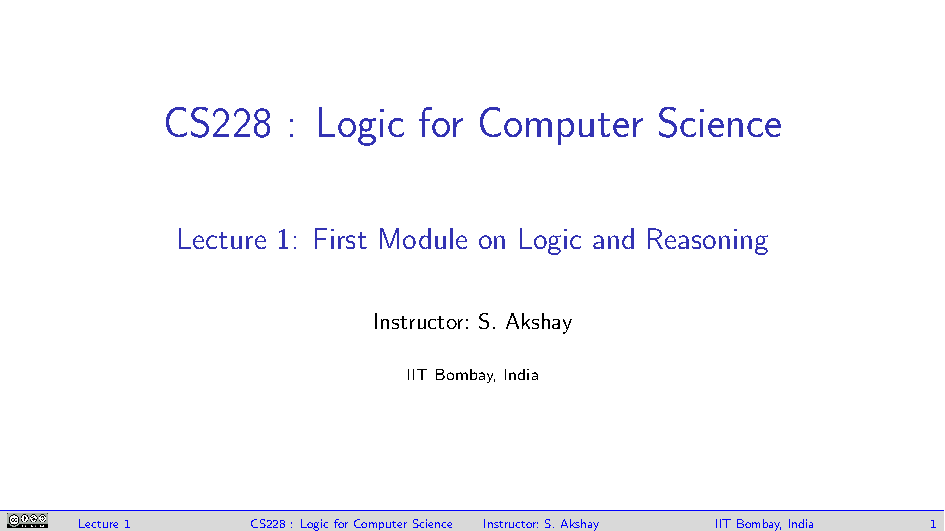
\includepdf[pages={1-4}]{CS228EndsemSlides.pdf} 
}
\subsection{Syntax and Parse Trees}
{
\setbeamercolor{background canvas}{bg=} % Prevents theme background from overlapping the PDF
\includepdf[pages={5-29}]{CS228EndsemSlides.pdf} 
}
\subsection{Semantics, Equivalence, Satisfiability and Validity}
{
\setbeamercolor{background canvas}{bg=} % Prevents theme background from overlapping the PDF
\includepdf[pages={30-51}]{CS228EndsemSlides.pdf} 
}
\subsection{Natural Deduction as a Proof System}
{
\setbeamercolor{background canvas}{bg=} % Prevents theme background from overlapping the PDF
\includepdf[pages={52-112}]{CS228EndsemSlides.pdf} 
}
\subsection{Normal Forms}
{
\setbeamercolor{background canvas}{bg=} % Prevents theme background from overlapping the PDF
\includepdf[pages={113-135}]{CS228EndsemSlides.pdf} 
}
\section{Module 2 : Satisfiability}

% 2. Insert pages from your external PDF here
% This will automatically break out of the Beamer layout to display the PDF pages full-screen.
{
\setbeamercolor{background canvas}{bg=} % Prevents theme background from overlapping the PDF
\includepdf[pages={136-140}]{CS228EndsemSlides.pdf} 
}
\subsection{Resolution Rule}
{
\setbeamercolor{background canvas}{bg=} % Prevents theme background from overlapping the PDF
\includepdf[pages={141-167}]{CS228EndsemSlides.pdf} 
}
\subsection{DPLL and CDCL}
{
\setbeamercolor{background canvas}{bg=} % Prevents theme background from overlapping the PDF
\includepdf[pages={168-224}]{CS228EndsemSlides.pdf} 
}
\section{Module 3 : Predicate Logic}

% 2. Insert pages from your external PDF here
% This will automatically break out of the Beamer layout to display the PDF pages full-screen.
{
\setbeamercolor{background canvas}{bg=} % Prevents theme background from overlapping the PDF
\includepdf[pages={225-228}]{CS228EndsemSlides.pdf} 
}
\subsection{Syntax and Semantics}
{
\setbeamercolor{background canvas}{bg=} % Prevents theme background from overlapping the PDF
\includepdf[pages={229-261}]{CS228EndsemSlides.pdf} 
}
\subsection{Natural Deduction}
{
\setbeamercolor{background canvas}{bg=} % Prevents theme background from overlapping the PDF
\includepdf[pages={262-280}]{CS228EndsemSlides.pdf} 
}
\subsection{Soundness, Completeness and Expressibility}
{
\setbeamercolor{background canvas}{bg=} % Prevents theme background from overlapping the PDF
\includepdf[pages={281-298}]{CS228EndsemSlides.pdf} 
}
\subsection{Normal Forms and Satisfiability Modulo Theories}
{
\setbeamercolor{background canvas}{bg=} % Prevents theme background from overlapping the PDF
\includepdf[pages={299-324}]{CS228EndsemSlides.pdf} 
}

\section{Module 4 : Hoare Logic}

% 2. Insert pages from your external PDF here
% This will automatically break out of the Beamer layout to display the PDF pages full-screen.
{
\setbeamercolor{background canvas}{bg=} % Prevents theme background from overlapping the PDF
\includepdf[pages={325-334}]{CS228EndsemSlides.pdf} 
}
\subsection{Syntax and Proof Calculus}
{
\setbeamercolor{background canvas}{bg=} % Prevents theme background from overlapping the PDF
\includepdf[pages={335-375}]{CS228EndsemSlides.pdf} 
}
\subsection{Total Correctness}
{
\setbeamercolor{background canvas}{bg=} % Prevents theme background from overlapping the PDF
\includepdf[pages={376-391}]{CS228EndsemSlides.pdf} 
}
\section{Module 5 : Temporal Logic}

% 2. Insert pages from your external PDF here
% This will automatically break out of the Beamer layout to display the PDF pages full-screen.
{
\setbeamercolor{background canvas}{bg=} % Prevents theme background from overlapping the PDF
\includepdf[pages={392-401}]{CS228EndsemSlides.pdf} 
}
\subsection{Models and Temporal Connectives}
{
\setbeamercolor{background canvas}{bg=} % Prevents theme background from overlapping the PDF
\includepdf[pages={402-409}]{CS228EndsemSlides.pdf} 
}
\subsection{LTL Syntax and Semantics}
{
\setbeamercolor{background canvas}{bg=} % Prevents theme background from overlapping the PDF
\includepdf[pages={410-429}]{CS228EndsemSlides.pdf} 
}
\subsection{CTL Syntax and Semantics}
{
\setbeamercolor{background canvas}{bg=} % Prevents theme background from overlapping the PDF
\includepdf[pages={430-442}]{CS228EndsemSlides.pdf} 
}
\subsection{Model Checking and Conclusion}
{
\setbeamercolor{background canvas}{bg=} % Prevents theme background from overlapping the PDF
\includepdf[pages={443-447}]{CS228EndsemSlides.pdf} 
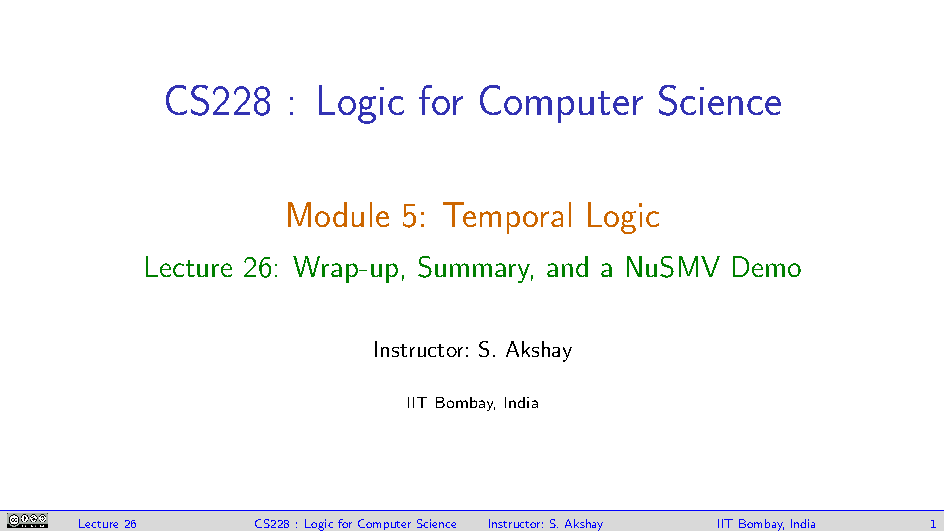
\includepdf[pages=-]{Lec-26.pdf}
}




\end{document}


